\section{Análisis de entidades}

   \paragraph{}Una entidad es un tipo de objeto definido mediante la agregación
   de una serie de atributos que se corresponde con la caracterización de
   objetos del mundo real, los cuales son definidos y diferenciados del resto de
   los objetos, sobre la base del conjunto de atributos que se agregan.

   \paragraph{}A continuación, se describirán los tipos de entidades a tratar
   por el sistema, describiendo para cada una de ellas sus características
   principales. Dichas entidades son:

   \begin{itemize}
    \item Entidad Centro.
    \item Entidad Administrador Centro.
    \item Entidad Titulación.
    \item Entidad Asignatura.
    \item Entidad Asignatura Curso Académico.
    \item Entidad Departamento.
    \item Entidad Asesor.
    \item Entidad Asesor Curso Académico.
    \item Entidad Plantilla Entrevista Asesor.
    \item Entidad Pregunta Asesor.
    \item Entidad Alumno.
    \item Entidad Alumno Curso Académico.
    \item Entidad Calificación Alumno Asignatura CA.
    \item Entidad Plantilla Entrevista Oficial.
    \item Entidad Pregunta Oficial.
    \item Entidad Reunión.
   \end{itemize}

   \paragraph{}Para la descripción de cada tipo de entidad, se utilizarán los
   siguientes apartados:

   \begin{description}
      \item[Definición] Especifica la función o el papel que desempeña el tipo
           de entidad en el mundo real. Además, también se describirán las
           posibles dependencias que tenga el tipo de entidad con otros
           existentes en el sistema.

      \item[Características] En este apartado se mostrará la siguiente
           información:

            \begin{itemize}
             \item Nombre de la entidad.
             \item Tipo de la entidad, es decir, fuerte, débil o subtipo de
                   entidad.
             \item Número de atributos.
             \item Atributo/s identificador/es principal/es.
             \item Atributo/s identificador/es alternativo/s.
             \item Atributo/s heredado/s.
            \end{itemize}

      \item[Diagrama] Representación gráfica del tipo de entidad.

      \item[Descripción de los atributos] Se describirán cada uno de los
           atributos que forman parte del tipo de entidad. Para cada uno de
           ellos, se indicará lo siguiente:

           \begin{itemize}
            \item Definición del atributo.
            \item Dominio en el cual se encuentra.
            \item Carácter del atributo, indicando si es opcional u obligatorio.
            \item Ejemplo práctico de cada atributo.
            \item Información adicional que sea interesante comentar.
           \end{itemize}

      \item[Ejemplo práctico del tipo de entidad] En este apartado se muestra
           una ocurrencia concreta del tipo de entidad.

   \end{description}

   \subsection{Tipo de entidad Centro}

   \begin{description}

   \item[Definición] Se refiere al objeto del mundo real: \emph{``Institución académica de la Universidad de Córdoba donde se imparten títulos universitarios''}.

   \item[Características] La entidad presenta las siguientes características:
      \begin{itemize}
         \item \textbf{Nombre:} Centro.
         \item \textbf{Tipo:} Fuerte.
         \item \textbf{Número de atributos:} 2.
         \item \textbf{Atributo/s identificador/es principal/es:} id\_centro.
         \item \textbf{Atributo/s identificador/es alternativo/s:} nombre\_centro.
         \item \textbf{Atributo/s heredado/s:} -
      \end{itemize}

   \item[Diagrama] La figura \ref{diagramaCentro} muestra el diagrama de la entidad.
   \item \begin{figure}[!ht]
            \begin{center}
            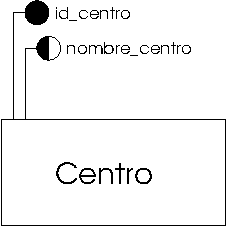
\includegraphics[]{07.Modelo_Entidad-Interrelacion/7.2.Analisis_Entidades/diagramas/centro.pdf}
            \caption{Diagrama de la entidad Centro.}
            \label{diagramaCentro}
            \end{center}
         \end{figure}

   \item[Descripción de los atributos] La entidad presenta los siguientes
   atributos:

   \begin{itemize}
    \item \textbf{id\_centro}
      \begin{itemize}
         \item \textbf{Definición:} Código que sirve como número identificativo
               para cada centro del sistema.
         \item \textbf{Dominio:} Números naturales.
         \item \textbf{Carácter:} Obligatorio.
         \item \textbf{Ejemplo práctico:} 15.
         \item \textbf{Información adicional:} El dato lo genera el sistema
               cuando el administrador principal introduce un nuevo centro en
               el sistema. Es la clave primaria.
      \end{itemize}
   \item \textbf{nombre\_centro}
      \begin{itemize}
         \item \textbf{Definición:} Denominación de un centro dentro del sistema.
         \item \textbf{Dominio:} Conjunto de caracteres alfanuméricos.
         \item \textbf{Carácter:} Obligatorio.
         \item \textbf{Ejemplo práctico:} Escuela Politécnica Superior.
         \item \textbf{Información adicional:} El dato lo introduce el
         administrador principal al introducir un nuevo centro en el sistema. Es
         clave alterna.
      \end{itemize}
   \end{itemize}

   \item[Ejemplo práctico]

   \item \begin{center}
            \begin{tabular}{ | l | l | }
            \hline
            \multicolumn{2}{ | c | }{\textbf{Tipo de entidad Centro}} \\
            \hline
            id\_centro & 15 \\
            \hline
            nombre\_centro & Escuela Politécnica Superior \\
            \hline
            \end{tabular}
         \end{center}
   \end{description}

   \subsection{Tipo de entidad Administrador Centro}

   \begin{description}

   \item[Definición] Se refiere al objeto del mundo real: \emph{``Individuo que
    gestiona la información relativa a un centro''}.

   \item[Características] La entidad presenta las siguientes características:
      \begin{itemize}
         \item \textbf{Nombre:} Administrador Centro.
         \item \textbf{Tipo:} Débil por existencia con respecto a Centro.
         \item \textbf{Número de atributos:} 2.
         \item \textbf{Atributo/s identificador/es principal/es:} id\_centro.
         \item \textbf{Atributo/s identificador/es alternativo/s:} -
         \item \textbf{Atributo/s heredado/s:} nombre\_centro, del tipo de
               entidad Centro.
      \end{itemize}

   \item[Diagrama]
   \item \begin{figure}[h!]
            \begin{center}
            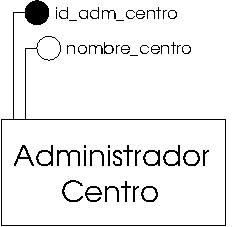
\includegraphics[]{07.Modelo_Entidad-Interrelacion/7.2.Analisis_Entidades/diagramas/adm_centro.pdf}
            \caption{Diagrama de la entidad Administrador Centro}
            \end{center}
         \end{figure}

   \item[Descripción de los atributos] La entidad presenta los siguientes
   atributos:

   \begin{itemize}
    \item \textbf{id\_adm\_centro}
      \begin{itemize}
         \item \textbf{Definición:} Código que sirve como número identificativo
               para cada usuario administrador de centro del sistema.
         \item \textbf{Dominio:} Números naturales.
         \item \textbf{Carácter:} Obligatorio.
         \item \textbf{Ejemplo práctico:} 9.
         \item \textbf{Información adicional:} El dato lo genera el sistema
               cuando el administrador principal introduce un nuevo usuario
               administrador de centro. Es la clave primaria.
      \end{itemize}
   \item \textbf{nombre\_centro}
      \begin{itemize}
         \item \textbf{Definición:} Denominación de un centro dentro del sistema.
         \item \textbf{Dominio:} Conjunto de caracteres alfanuméricos.
         \item \textbf{Carácter:} Obligatorio.
         \item \textbf{Ejemplo práctico:} Escuela Politécnica Superior.
         \item \textbf{Información adicional:} El dato se hereda de la entidad
               Centro.
      \end{itemize}
   \end{itemize}

   \item[Ejemplo práctico]

   \item \begin{center}
            \begin{tabular}{ | l | l | }
            \hline
            \multicolumn{2}{ | c | }{\textbf{Tipo de entidad Administrador Centro}} \\
            \hline
            id\_adm\_centro & 9 \\
            \hline
            nombre\_centro & Escuela Politécnica Superior \\
            \hline
            \end{tabular}
         \end{center}
   \end{description}

   \subsection{Tipo de entidad Titulación}

   \begin{description}

   \item[Definición] Se refiere al objeto del mundo real: \emph{``Conjunto de
        materias cuya superación supone la obtención de un título académico''}.

   \item[Características] La entidad presenta las siguientes características:
      \begin{itemize}
         \item \textbf{Nombre:} Titulación.
         \item \textbf{Tipo:} Fuerte.
         \item \textbf{Número de atributos:} 2.
         \item \textbf{Atributo/s identificador/es principal/es:} id\_titulacion.
         \item \textbf{Atributo/s identificador/es alternativo/s:} nombre\_titulacion
         \item \textbf{Atributo/s heredado/s:} -
      \end{itemize}

   \item[Diagrama]
   \item \begin{figure}[h!]
            \begin{center}
            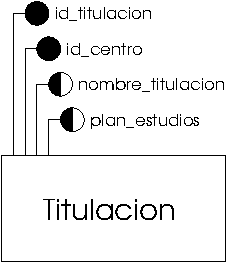
\includegraphics[]{07.Modelo_Entidad-Interrelacion/7.2.Analisis_Entidades/diagramas/titulacion.pdf}
            \caption{Diagrama de la entidad Titulación}
            \end{center}
         \end{figure}

   \item[Descripción de los atributos] La entidad presenta los siguientes
   atributos:

   \begin{itemize}
    \item \textbf{id\_titulacion}
      \begin{itemize}
         \item \textbf{Definición:} Código que sirve como número identificativo
         para cada titulación dentro del sistema.
         \item \textbf{Dominio:} Números naturales.
         \item \textbf{Carácter:} Obligatorio.
         \item \textbf{Ejemplo práctico:} 3.
         \item \textbf{Información adicional:} El dato lo genera el sistema
         cuando el administrador introduce la titulación en el sistema.
         Es la clave primaria.
      \end{itemize}
   \item \textbf{nombre\_titulacion}
      \begin{itemize}
         \item \textbf{Definición:} Denominación de una titulación dentro del sistema.
         \item \textbf{Dominio:} Conjunto de caracteres alfanuméricos.
         \item \textbf{Carácter:} Obligatorio.
         \item \textbf{Ejemplo práctico:} Ingeniería Técnica en Informática de Gestión.
         \item \textbf{Información adicional:} El dato lo proporciona el administrador en el momento de introducir la titulación en el sistema. Es la clave alterna
      \end{itemize}
   \end{itemize}

   \item[Ejemplo práctico]

   \item \begin{center}
            \begin{tabular}{ | l | l | }
            \hline
            \multicolumn{2}{ | c | }{\textbf{Tipo de entidad Titulación}} \\
            \hline
            id\_centro & 3 \\
            \hline
            nombre\_centro & Ingeniería Técnica en Informática de Gestión \\
            \hline
            \end{tabular}
         \end{center}
   \end{description}

   \subsection{Tipo de entidad Asignatura}

   \begin{description}

   \item[Definición] Se refiere al objeto del mundo real: \emph{``Materia que
   forma parte del plan de estudios de una titulación''}.

   \item[Características] La entidad presenta las siguientes características:
      \begin{itemize}
         \item \textbf{Nombre:} Asignatura.
         \item \textbf{Tipo:} Débil por identificación con respecto a Titulación.
         \item \textbf{Número de atributos:} 8.
         \item \textbf{Atributo/s identificador/es principal/es:} id\_centro junto con \\id\_titulación e id\_asignatura.
         \item \textbf{Atributo/s identificador/es alternativo/s:} id\_centro junto con \\id\_titulación y nombre\_asignatura.
         \item \textbf{Atributo/s heredado/s:} id\_centro del tipo de entidad Centro, \\id\_titulación del tipo de entidad Titulación.
      \end{itemize}

   \item[Diagrama] La figura \ref{diagramaAsignatura} muestra el diagrama de la entidad.
   \item \begin{figure}[!ht]
            \begin{center}
            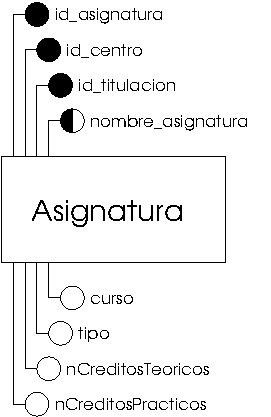
\includegraphics[]{07.Modelo_Entidad-Interrelacion/7.2.Analisis_Entidades/diagramas/asignatura.pdf}
            \caption{Diagrama de la entidad Asignatura.}
            \label{diagramaAsignatura}
            \end{center}
         \end{figure}

   \item[Descripción de los atributos] La entidad presenta los siguientes
   atributos:

   \begin{itemize}
   \item \textbf{id\_centro}
      \begin{itemize}
         \item \textbf{Definición:} Código que sirve como número identificativo
               para cada centro del sistema.
         \item \textbf{Dominio:} Números naturales.
         \item \textbf{Carácter:} Obligatorio.
         \item \textbf{Ejemplo práctico:} 15.
         \item \textbf{Información adicional:} El dato se hereda del tipo de
         entidad Centro. Es la clave primaria junto con id\_titulación e
         id\_asignatura. También actúa de clave alterna junto con
         id\_titulación y nombre\_asignatura.
      \end{itemize}
   \item \textbf{id\_titulación}
      \begin{itemize}
         \item \textbf{Definición:} Código que sirve como número identificativo
         para cada titulación dentro del sistema.
         \item \textbf{Dominio:} Números naturales.
         \item \textbf{Carácter:} Obligatorio.
         \item \textbf{Ejemplo práctico:} 3.
         \item \textbf{Información adicional:} El dato se hereda del tipo de
         entidad Titulación. Es la clave primaria junto con id\_centro e
         id\_asignatura. También actúa de clave alterna junto con
         id\_centro y nombre\_asignatura.
      \end{itemize}
   \item \textbf{id\_asignatura}
      \begin{itemize}
         \item \textbf{Definición:} Código que sirve como número identificativo
         para cada asignatura dentro del sistema.
         \item \textbf{Dominio:} Números naturales.
         \item \textbf{Carácter:} Obligatorio.
         \item \textbf{Ejemplo práctico:} 17.
         \item \textbf{Información adicional:} El dato lo proporciona el sistema, cuando el administrador, principal o de centro, introduce la asignatura en el sistema. Es la clave primaria junto con id\_centro y con id\_titulación.
      \end{itemize}
   \item \textbf{nombre\_asignatura}
      \begin{itemize}
         \item \textbf{Definición:} Denominación de una asignatura dentro del sistema.
         \item \textbf{Dominio:} Conjunto de caracteres alfanuméricos.
         \item \textbf{Carácter:}  Obligatorio.
         \item \textbf{Ejemplo práctico:} Lenguajes de Inteligencia Artificial.
         \item \textbf{Información adicional:} El dato lo proporciona el administrador, principal o de
         centro, en el momento de introducir la asignatura en el sistema. Es la clave alterna junto con
         id\_centro y con id\_titulación.
      \end{itemize}
   \item \textbf{curso}
      \begin{itemize}
         \item \textbf{Definición:} Nivel académico de la asignatura en una titulación.
         \item \textbf{Dominio:} Números naturales.
         \item \textbf{Carácter:}  Opcional.
         \item \textbf{Ejemplo práctico:} 2.
         \item \textbf{Información adicional:} El dato lo proporciona el administrador, principal o de
         centro, en el momento de introducir la asignatura en el sistema.
      \end{itemize}
   \item \textbf{tipo}
      \begin{itemize}
         \item \textbf{Definición:} Clasificación de la asignatura según su tipo.
         \item \textbf{Dominio:} Uno de los valores: Troncal, Obligatoria, Optativa o Libre Configuración.
         \item \textbf{Carácter:}  Opcional.
         \item \textbf{Ejemplo práctico:} Optativa.
         \item \textbf{Información adicional:} El dato lo proporciona el administrador, principal o de
         centro, en el momento de introducir la asignatura en el sistema.
      \end{itemize}
   \item \textbf{nCréditosTeóricos}
      \begin{itemize}
         \item \textbf{Definición:} Valor relacionado con el número de horas que se estima necesario para dedicar al contenido teórico de una asignatura.
         \item \textbf{Dominio:} Números reales positivos.
         \item \textbf{Carácter:}  Opcional.
         \item \textbf{Ejemplo práctico:} 3.0.
         \item \textbf{Información adicional:} El dato lo proporciona el administrador, principal o de
         centro, en el momento de introducir la asignatura en el sistema.
      \end{itemize}
   \item \textbf{nCréditosPrácticos}
      \begin{itemize}
         \item \textbf{Definición:} Valor relacionado con el número de horas que se estima necesario para dedicar al contenido práctico de una asignatura.
         \item \textbf{Dominio:} Números reales positivos.
         \item \textbf{Carácter:}  Opcional.
         \item \textbf{Ejemplo práctico:} 1.5.
         \item \textbf{Información adicional:} El dato lo proporciona el administrador, principal o de
         centro, en el momento de introducir la asignatura en el sistema.
      \end{itemize}

   \end{itemize}

   \item[Ejemplo práctico]

   \item \begin{center}
            \begin{tabular}{ | l | l | }
            \hline
            \multicolumn{2}{ | c | }{\textbf{Tipo de entidad Asignatura}} \\
            \hline
            id\_centro & 15 \\
            \hline
            id\_titulación & 3\\
            \hline
            id\_asignatura & 17\\
            \hline
            nombre\_asignatura & Lenguajes de Inteligencia Artificial\\
            \hline
            curso & 2\\
            \hline
            tipo & Optativa\\
            \hline
            nCréditosTeóricos & 3.0\\
            \hline
            nCréditosPrácticos & 1.5\\
            \hline
            \end{tabular}
         \end{center}
   \end{description}

   \subsection{Tipo de entidad Asignatura Curso Académico}

   \begin{description}

   \item[Definición] Se refiere al objeto del mundo real: \emph{``Asignatura
   impartida en un determinado curso académico''}.

   \item[Características] La entidad presenta las siguientes características:
      \begin{itemize}
         \item \textbf{Nombre:} Asignatura Curso Académico.
         \item \textbf{Tipo:} Débil por identificación con respecto a Asignatura.
         \item \textbf{Número de atributos:} 1 propio y 3 heredados.
         \item \textbf{Atributo/s identificador/es principal/es:} id\_centro junto con \\id\_titulación, id\_asignatura y curso\_académico.
         \item \textbf{Atributo/s identificador/es alternativo/s:} -
         \item \textbf{Atributo/s heredado/s:} id\_centro, id\_titulación e
         id\_asignatura del tipo de entidad Asignatura.
      \end{itemize}

   \item[Diagrama] La figura \ref{diagramaACA} muestra el diagrama de la entidad.
   \item \begin{figure}[!ht]
            \begin{center}
            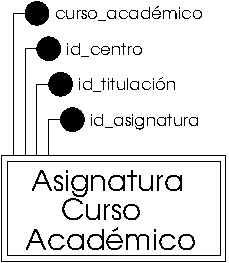
\includegraphics[]{07.Modelo_Entidad-Interrelacion/7.2.Analisis_Entidades/diagramas/aca.pdf}
            \caption{Diagrama de la entidad Asignatura Curso Académico.}
            \label{diagramaACA}
            \end{center}
         \end{figure}

   \item[Descripción de los atributos propios] La entidad presenta los
   siguientes atributos propios:

   \begin{itemize}
   \item \textbf{curso\_académico}
      \begin{itemize}
         \item \textbf{Definición:} Hace referencia al periodo de tiempo en que se imparte una determinada asignatura.
         \item \textbf{Dominio:} Formato de fecha: aaaa.
         \item \textbf{Carácter:}  Obligatorio.
         \item \textbf{Ejemplo práctico:} 2008.
         \item \textbf{Información adicional:} El dato lo proporciona el usuario alumno al establecer las asignaturas en las cuales se ha matriculado. Es la clave primaria junto con id\_centro, id\_titulación e id\_asignatura.
      \end{itemize}
   \end{itemize}

   \item[Ejemplo práctico]

   \item \begin{center}
            \begin{tabular}{ | l | l | }
            \hline
            \multicolumn{2}{ | c | }{\textbf{Tipo de entidad Asignatura Curso Académico}} \\
            \hline
            id\_centro & 15 \\
            \hline
            id\_titulación & 3\\
            \hline
            id\_asignatura & 17\\
            \hline
            curso\_académico & 2008\\
            \hline
            \end{tabular}
         \end{center}
   \end{description}

   \subsection{Tipo de entidad Departamento}

   \begin{description}

   \item[Definición] Se refiere al objeto del mundo real: \emph{``Unidad
   estructural universitaria de docencia e investigación, formada por una o
   varias cátedras de materias afines''}.

   \item[Características] La entidad presenta las siguientes características:
      \begin{itemize}
         \item \textbf{Nombre:} Departamento.
         \item \textbf{Tipo:} Fuerte.
         \item \textbf{Número de atributos:} 2.
         \item \textbf{Atributo/s identificador/es principal/es:} id\_departamento.
         \item \textbf{Atributo/s identificador/es alternativo/s:} nombre\_departamento.
         \item \textbf{Atributo/s heredado/s:} -
      \end{itemize}

   \item[Diagrama] La figura \ref{diagramaDepartamento} muestra el diagrama de la entidad.
   \item \begin{figure}[!ht]
            \begin{center}
            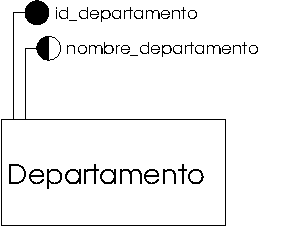
\includegraphics[]{07.Modelo_Entidad-Interrelacion/7.2.Analisis_Entidades/diagramas/departamento.pdf}
            \caption{Diagrama de la entidad Departamento.}
            \label{diagramaDepartamento}
            \end{center}
         \end{figure}

   \item[Descripción de los atributos] La entidad presenta los siguientes
   atributos:

   \begin{itemize}
    \item \textbf{id\_departamento}
      \begin{itemize}
         \item \textbf{Definición:} Código que sirve como número identificativo
               para cada departamento del sistema.
         \item \textbf{Dominio:} Números naturales.
         \item \textbf{Carácter:} Obligatorio.
         \item \textbf{Ejemplo práctico:} 22.
         \item \textbf{Información adicional:} El dato lo genera el sistema
               cuando el administrador principal introduce un nuevo departamento
               en el sistema. Es la clave primaria.
      \end{itemize}
   \item \textbf{nombre\_departamento}
      \begin{itemize}
         \item \textbf{Definición:} Denominación de un departamento dentro del sistema.
         \item \textbf{Dominio:} Conjunto de caracteres alfanuméricos.
         \item \textbf{Carácter:} Obligatorio.
         \item \textbf{Ejemplo práctico:} Departamento de Informática y Análisis Numérico.
         \item \textbf{Información adicional:} El dato lo introduce el
         administrador principal al introducir un nuevo departamento en el sistema. Es
         clave alterna.
      \end{itemize}
   \end{itemize}

   \item[Ejemplo práctico]

   \item \begin{center}
            \begin{tabular}{ | l | l | }
            \hline
            \multicolumn{2}{ | c | }{\textbf{Tipo de entidad Departamento}} \\
            \hline
            id\_departamento & 22 \\
            \hline
            nombre\_departamento & Departamento de Informática y Análisis Numérico \\
            \hline
            \end{tabular}
         \end{center}
   \end{description}

   \subsection{Tipo de entidad Asesor}

   \begin{description}

   \item[Definición] Se refiere a la persona del mundo real: \emph{``Tutor que
        realiza un seguimiento permanente y orientado a la optimización del
        esfuerzo de estudio de un alumno en un curso académico''}.

   \item[Características] La entidad presenta las siguientes características:
      \begin{itemize}
         \item \textbf{Nombre:} Asesor.
         \item \textbf{Tipo:} Fuerte.
         \item \textbf{Número de atributos:} 4.
         \item \textbf{Atributo/s identificador/es principal/es:} dni\_pasaporte.
         \item \textbf{Atributo/s identificador/es alternativo/s:} correo\_electronico.
         \item \textbf{Atributo/s heredado/s:} -
      \end{itemize}

   \item[Diagrama] La figura \ref{diagramaAsesor} muestra el diagrama de la entidad.
   \item \begin{figure}[!ht]
            \begin{center}
            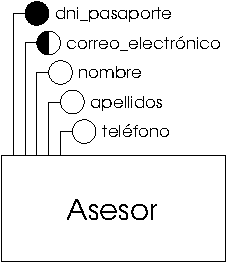
\includegraphics[]{07.Modelo_Entidad-Interrelacion/7.2.Analisis_Entidades/diagramas/asesor.pdf}
            \caption{Diagrama de la entidad Asesor.}
            \label{diagramaAsesor}
            \end{center}
         \end{figure}

   \item[Descripción de los atributos] La entidad presenta los siguientes
   atributos:

   \begin{itemize}
   \item \textbf{dni\_pasaporte}
      \begin{itemize}
         \item \textbf{Definición:} Coincide con el documento nacional de identidad o pasaporte de la persona.
         \item \textbf{Dominio:} Conjunto de caracteres alfanuméricos.
         \item \textbf{Carácter:} Obligatorio.
         \item \textbf{Ejemplo práctico:} 98765432Z.
         \item \textbf{Información adicional:} El dato lo proporciona el administrador, principal o de centro, cuando introduce al usuario asesor en el sistema. Es la clave primaria.
      \end{itemize}
   \item \textbf{correo\_electrónico}
      \begin{itemize}
         \item \textbf{Definición:} Contiene la dirección de correo electrónico de la persona.
         \item \textbf{Dominio:} Conjunto de caracteres alfanuméricos permitidos en una dirección de correo electrónico.
         \item \textbf{Carácter:} Opcional.
         \item \textbf{Ejemplo práctico:} ma1fegan@uco.es
         \item \textbf{Información adicional:} El dato lo proporciona o bien el usuario administrador, principal o de centro, cuando registra al asesor en el sistema, o bien el propio usuario asesor cuando modifica su información personal. Es la clave alterna.
      \end{itemize}
   \item \textbf{nombre}
      \begin{itemize}
         \item \textbf{Definición:} Designa el nombre de pila del usuario asesor que interviene en el sistema.
         \item \textbf{Dominio:} Conjunto de caracteres alfanuméricos.
         \item \textbf{Carácter:} Obligatorio.
         \item \textbf{Ejemplo práctico:} Nicolás Luis.
         \item \textbf{Información adicional:} El dato lo proporciona o bien el usuario administrador, principal o de centro, cuando registra al asesor en el sistema, o bien el propio usuario asesor cuando modifica su información personal.
      \end{itemize}
   \item \textbf{apellidos}
      \begin{itemize}
         \item \textbf{Definición:} Hace referencia a los apellidos del usuario asesor que interviene en el sistema.
         \item \textbf{Dominio:} Conjunto de caracteres alfanuméricos.
         \item \textbf{Carácter:}  Opcional.
         \item \textbf{Ejemplo práctico:} Fernández García.
         \item \textbf{Información adicional:} El dato lo proporciona o bien el usuario administrador, principal o de centro, cuando registra al asesor en el sistema, o bien el propio usuario asesor cuando modifica su información personal.
      \end{itemize}
   \end{itemize}

   \item[Ejemplo práctico]

   \item \begin{center}
            \begin{tabular}{ | l | l | }
            \hline
            \multicolumn{2}{ | c | }{\textbf{Tipo de entidad Asesor}} \\
            \hline
            dni\_pasaporte & 98765432Z \\
            \hline
            correo\_electrónico & ma1fegan@uco.es\\
            \hline
            nombre & Nicolás Luis\\
            \hline
            apellidos & Fernández García\\
            \hline
            \end{tabular}
         \end{center}
   \end{description}

   \subsection{Tipo de entidad Asesor Curso Académico}

   \begin{description}

   \item[Definición] Se refiere al objeto del mundo real: \emph{``Asesor
   que realiza labor de tutoría durante un curso académico''}.

   \item[Características] La entidad presenta las siguientes características:
      \begin{itemize}
         \item \textbf{Nombre:} Asesor Curso Académico.
         \item \textbf{Tipo:} Débil por identificación con respecto a Asesor y débil por existencia respecto a Departamento.
         \item \textbf{Número de atributos:} 1 propio y 1 heredado.
         \item \textbf{Atributo/s identificador/es principal/es:} dni\_pasaporte y \\curso\_académico.
         \item \textbf{Atributo/s identificador/es alternativo/s:} -
         \item \textbf{Atributo/s heredado/s:} dni\_pasaporte del tipo
         de entidad Asesor.
      \end{itemize}

   \item[Diagrama] La figura \ref{diagramaAsesorCA} muestra el diagrama de la entidad.
   \item \begin{figure}[!ht]
            \begin{center}
            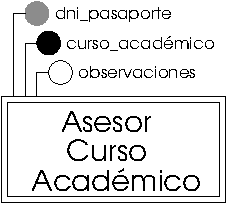
\includegraphics[]{07.Modelo_Entidad-Interrelacion/7.2.Analisis_Entidades/diagramas/asesorca.pdf}
            \caption{Diagrama de la entidad Asesor Curso Académico.}
            \label{diagramaAsesorCA}
            \end{center}
         \end{figure}

   \item[Descripción de los atributos propios] Esta entidad presenta el
   siguiente atributo propio:

   \begin{itemize}
   \item \textbf{curso\_académico}
      \begin{itemize}
         \item \textbf{Definición:} Hace referencia al periodo de tiempo en que se imparte una determinada asignatura.
         \item \textbf{Dominio:} Formato de fecha: aaaa.
         \item \textbf{Carácter:}  Obligatorio.
         \item \textbf{Ejemplo práctico:} 2007.
         \item \textbf{Información adicional:} El dato \textit{¿quién lo proporciona?}. Es la clave primaria junto con dni\_pasaporte.
      \end{itemize}
   \end{itemize}

   \item[Ejemplo práctico]

   \item \begin{center}
            \begin{tabular}{ | l | l | }
            \hline
            \multicolumn{2}{ | c | }{\textbf{Tipo de entidad Asesor Curso Académico}} \\
            \hline
            dni\_pasaporte & 98765432Z \\
            \hline
            curso\_académico & 2007\\
            \hline
            \end{tabular}
         \end{center}
   \end{description}

   \subsection{Tipo de entidad Plantilla Entrevista Asesor}

   \begin{description}

   \item[Definición] Se refiere al objeto del mundo real: \emph{``Conjunto de
   preguntas predefinidas por un asesor que pueden ser utilizadas por éste
   durante una reunión con un alumno''}.

   \item[Características] La entidad presenta las siguientes características:
      \begin{itemize}
         \item \textbf{Nombre:} Plantilla Entrevista Asesor.
         \item \textbf{Tipo:} Fuerte.
         \item \textbf{Número de atributos:} 3 propios y 2 heredados.
         \item \textbf{Atributo/s identificador/es principal/es:} dni\_pasaporte
         junto con curso\_académico e id\_entrevista\_asesor.
         \item \textbf{Atributo/s identificador/es alternativo/s:} -
         \item \textbf{Atributo/s heredado/s:} dni\_pasaporte y curso\_académico
         del tipo de entidad Asesor Curso Académico.
      \end{itemize}

   \item[Diagrama] La figura \ref{diagramaPlantEntAse} muestra el diagrama de la entidad.
   \item \begin{figure}[!ht]
            \begin{center}
            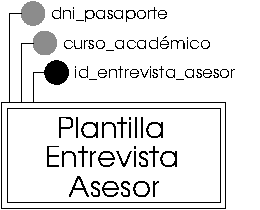
\includegraphics[]{07.Modelo_Entidad-Interrelacion/7.2.Analisis_Entidades/diagramas/plant_ent_ase.pdf}
            \caption{Diagrama de la entidad Plantilla Entrevista Asesor.}
            \label{diagramaPlantEntAse}
            \end{center}
         \end{figure}

   \item[Descripción de los atributos propios] La entidad presenta los
   siguientes atributos propios:

   \begin{itemize}
    \item \textbf{id\_entrevista\_asesor}
      \begin{itemize}
         \item \textbf{Definición:} Código que sirve como número identificativo
               para cada plantilla de entrevista de asesor del sistema.
         \item \textbf{Dominio:} Números naturales.
         \item \textbf{Carácter:} Obligatorio.
         \item \textbf{Ejemplo práctico:} 36.
         \item \textbf{Información adicional:} El dato lo genera el sistema
               cuando se introduce una nueva plantilla de entrevista de asesor
               en el sistema. Es la clave primaria.
      \end{itemize}
    \item \textbf{descripción}
      \begin{itemize}
         \item \textbf{Definición:} Establece una breve descripción que permite
         reconocer una plantilla de entrevista de asesor del resto.
         \item \textbf{Dominio:} Conjunto de caracteres alfanuméricos.
         \item \textbf{Carácter:} Opcional.
         \item \textbf{Ejemplo práctico:} Plantilla sobre prácticas.
         \item \textbf{Información adicional:} El dato lo introduce el
         usuario asesor al introducir una nueva plantilla de entrevista de
         asesor en el sistema.
      \end{itemize}
    \item \textbf{última\_modificación}
      \begin{itemize}
         \item \textbf{Definición:} Establece el día, mes y año cuando se
            produjo la última modificación de la entidad.
         \item \textbf{Dominio:} Formato de fecha: dd/mm/aaaa.
         \item \textbf{Carácter:} Opcional.
         \item \textbf{Ejemplo práctico:} 02/02/2009.
         \item \textbf{Información adicional:} El dato lo genera el sistema
               cuando se modifica una plantilla de entrevista de asesor en
               el sistema.
      \end{itemize}
   \end{itemize}

   \item[Ejemplo práctico]

   \item \begin{center}
            \begin{tabular}{ | l | l | }
            \hline
            \multicolumn{2}{ | c | }{\textbf{Tipo de entidad Plantilla Entrevista Asesor}} \\
            \hline
            dni\_pasaporte & 98765432Z \\
            \hline
            curso\_académico & 2008 \\
            \hline
            id\_entrevista\_asesor & 36 \\
            \hline
            descripción & Plantilla sobre prácticas \\
            \hline
            última\_modificación & 02/02/2009 \\
            \hline
            \end{tabular}
         \end{center}
   \end{description}

   \subsection{Tipo de entidad Pregunta Asesor}

   \begin{description}

   \item[Definición] Se refiere al objeto del mundo real: \emph{``Cuestión
   perteneciente a una plantilla de entrevista de asesor planteada por el
   usuario asesor al usuario alumno''}.

   \item[Características] La entidad presenta las siguientes características:
      \begin{itemize}
         \item \textbf{Nombre:} Pregunta Asesor.
         \item \textbf{Tipo:} Débil por identificación con respecto a
         Plantilla Entrevista Asesor.
         \item \textbf{Número de atributos:} 2 propios y 3 heredados.
         \item \textbf{Atributo/s identificador/es principal/es:} id\_pregunta\_oficial.
         \item \textbf{Atributo/s identificador/es alternativo/s:} -
         \item \textbf{Atributo/s heredado/s:} dni\_pasaporte, curso\_académico
         además del atributo id\_entrevista\_asesor del tipo de entidad
         Plantilla Entrevista Asesor.
      \end{itemize}

   \item[Diagrama] La figura \ref{diagramaPregAse} muestra el diagrama de la entidad.
   \item \begin{figure}[!ht]
            \begin{center}
            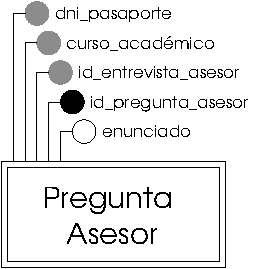
\includegraphics[]{07.Modelo_Entidad-Interrelacion/7.2.Analisis_Entidades/diagramas/preg_ase.pdf}
            \caption{Diagrama de la entidad Pregunta Asesor.}
            \label{diagramaPregAse}
            \end{center}
         \end{figure}

   \item[Descripción de los atributos propios] La entidad presenta los siguientes
   atributos propios:

   \begin{itemize}
    \item \textbf{id\_pregunta\_asesor}
      \begin{itemize}
         \item \textbf{Definición:} Código que sirve como número identificativo
               para cada pregunta de asesor del sistema.
         \item \textbf{Dominio:} Números naturales.
         \item \textbf{Carácter:} Obligatorio.
         \item \textbf{Ejemplo práctico:} 72.
         \item \textbf{Información adicional:} El dato lo genera el sistema
               cuando se introduce una nueva pregunta de asesor en el sistema.
               Es la clave primaria.
      \end{itemize}
   \item \textbf{enunciado}
      \begin{itemize}
         \item \textbf{Definición:} Cuestión perteneciente a una entrevista
         de asesor, planteada a un alumno.
         \item \textbf{Dominio:} Conjunto de caracteres alfanuméricos.
         \item \textbf{Carácter:} Obligatorio.
         \item \textbf{Ejemplo práctico:} Nivel de inglés.
         \item \textbf{Información adicional:} El dato lo introduce el
         usuario administrador al introducir una nueva pregunta de asesor en
         el sistema.
      \end{itemize}
   \end{itemize}

   \item[Ejemplo práctico]

   \item \begin{center}
            \begin{tabular}{ | l | l | }
            \hline
            \multicolumn{2}{ | c | }{\textbf{Tipo de entidad Pregunta Asesor}} \\
            \hline
            dni\_pasaporte & 98765432Z \\
            \hline
            curso\_académico & 2008 \\
            \hline
            id\_entrevista\_asesor & 36 \\
            \hline
            id\_pregunta\_asesor & 72 \\
            \hline
            enunciado & Nivel de inglés \\
            \hline
            \end{tabular}
         \end{center}
   \end{description}

   \subsection{Tipo de entidad Alumno}

   \begin{description}

   \item[Definición] Se refiere a la persona del mundo real: \emph{``Estudiante
        de una titulación que recibe asesoría''}.

   \item[Características] La entidad presenta las siguientes características:
      \begin{itemize}
         \item \textbf{Nombre:} Alumno.
         \item \textbf{Tipo:} Fuerte.
         \item \textbf{Número de atributos:} 19.
         \item \textbf{Atributo/s identificador/es principal/es:} dni\_pasaporte.
         \item \textbf{Atributo/s identificador/es alternativo/s:} correo\_electrónico.
         \item \textbf{Atributo/s heredado/s:} -
      \end{itemize}

   \item[Diagrama] La figura \ref{diagramaAlumno} muestra el diagrama de la entidad.
   \item \begin{figure}[!ht]
            \begin{center}
            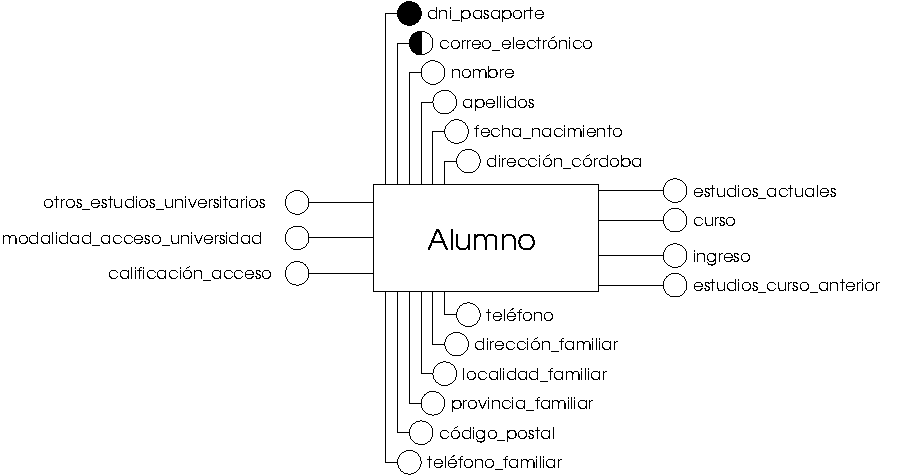
\includegraphics[]{07.Modelo_Entidad-Interrelacion/7.2.Analisis_Entidades/diagramas/alumno.pdf}
            \caption{Diagrama de la entidad Alumno.}
            \label{diagramaAlumno}
            \end{center}
         \end{figure}

   \item[Descripción de los atributos] La entidad presenta los siguientes
   atributos:

   \begin{itemize}
   \item \textbf{dni\_pasaporte}
      \begin{itemize}
         \item \textbf{Definición:} Coincide con el número de documento nacional
         de identidad o pasaporte del alumno.
         \item \textbf{Dominio:} Conjunto de caracteres alfanuméricos.
         \item \textbf{Carácter:} Obligatorio.
         \item \textbf{Ejemplo práctico:} 01234567A.
         \item \textbf{Información adicional:} El dato lo proporciona el usuario alumno, bien a la hora de registrarse, o bien cuando cuando modifica su información personal. Es la clave primaria.
      \end{itemize}
   \item \textbf{correo\_electrónico}
      \begin{itemize}
         \item \textbf{Definición:} Contiene la dirección de correo electrónico de la persona.
         \item \textbf{Dominio:} Conjunto de caracteres alfanuméricos permitidos en una dirección de correo electrónico.
         \item \textbf{Carácter:} Obligatorio.
         \item \textbf{Ejemplo práctico:} i42sasab@uco.es
         \item \textbf{Información adicional:} El dato lo proporciona el usuario alumno cuando se registra o cuando modifica su información personal. Es la clave alterna.
      \end{itemize}
   \item \textbf{nombre}
      \begin{itemize}
         \item \textbf{Definición:} Designa el nombre de pila del usuario alumno que interviene en el sistema.
         \item \textbf{Dominio:} Conjunto de caracteres alfanuméricos.
         \item \textbf{Carácter:} Obligatorio.
         \item \textbf{Ejemplo práctico:} Bartolomé.
         \item \textbf{Información adicional:} El dato lo proporciona el usuario alumno cuando se registra o cuando modifica su información personal.
      \end{itemize}
   \item \textbf{apellidos}
      \begin{itemize}
         \item \textbf{Definición:} Hace referencia a los apellidos del usuario alumno que interviene en el sistema.
         \item \textbf{Dominio:} Conjunto de caracteres alfanuméricos.
         \item \textbf{Carácter:}  Obligatorio.
         \item \textbf{Ejemplo práctico:} Sánchez Salado.
         \item \textbf{Información adicional:} El dato lo proporciona el usuario alumno cuando se registra o cuando modifica su información personal.
      \end{itemize}
   \item \textbf{fecha\_nacimiento}
      \begin{itemize}
         \item \textbf{Definición:} Contiene la fecha de nacimiento del alumno.
         \item \textbf{Dominio:} Formato de fecha: dd-mm-aaaa.
         \item \textbf{Carácter:}  Opcional.
         \item \textbf{Ejemplo práctico:} 13-12-1984.
         \item \textbf{Información adicional:} El dato lo proporciona el usuario alumno cuando se registra o cuando modifica su información personal.
      \end{itemize}
   \item \textbf{dirección\_córdoba}
      \begin{itemize}
         \item \textbf{Definición:} Hace referencia a la dirección del alumno durante el curso.
         \item \textbf{Dominio:} Conjunto de caracteres alfanuméricos.
         \item \textbf{Carácter:}  Opcional.
         \item \textbf{Ejemplo práctico:} 13 Rue del Percebe.
         \item \textbf{Información adicional:} El dato lo proporciona el usuario alumno cuando se registra o cuando modifica su información personal.
      \end{itemize}
   \item \textbf{teléfono}
      \begin{itemize}
         \item \textbf{Definición:} Hace referencia a un número de teléfono perteneciente al alumno.
         \item \textbf{Dominio:} Conjunto de enteros positivos.
         \item \textbf{Carácter:}  Opcional.
         \item \textbf{Ejemplo práctico:} 601234567.
         \item \textbf{Información adicional:} El dato lo proporciona el usuario alumno cuando se registra o cuando modifica su información personal.
      \end{itemize}
   \item \textbf{dirección\_familiar}
      \begin{itemize}
         \item \textbf{Definición:} Hace referencia a la dirección del domicilio familiar del alumno.
         \item \textbf{Dominio:} Conjunto de caracteres alfanuméricos.
         \item \textbf{Carácter:}  Opcional.
         \item \textbf{Ejemplo práctico:} Calle Edsger Dijkstra, 30.
         \item \textbf{Información adicional:} El dato lo proporciona el usuario alumno cuando se registra o cuando modifica su información personal.
      \end{itemize}
   \item \textbf{localidad\_familiar}
      \begin{itemize}
         \item \textbf{Definición:} Hace referencia a la localidad del domicilio familiar del alumno.
         \item \textbf{Dominio:} Conjunto de caracteres alfanuméricos.
         \item \textbf{Carácter:}  Opcional.
         \item \textbf{Ejemplo práctico:} La Carlota.
         \item \textbf{Información adicional:} El dato lo proporciona el usuario alumno cuando se registra o cuando modifica su información personal.
      \end{itemize}
   \item \textbf{provincia\_familiar}
      \begin{itemize}
         \item \textbf{Definición:} Hace referencia a la provincia del domicilio familiar del alumno.
         \item \textbf{Dominio:} Conjunto de caracteres alfanuméricos.
         \item \textbf{Carácter:}  Opcional.
         \item \textbf{Ejemplo práctico:} Córdoba.
         \item \textbf{Información adicional:} El dato lo proporciona el usuario alumno cuando se registra o cuando modifica su información personal.
      \end{itemize}
   \item \textbf{código\_postal}
      \begin{itemize}
         \item \textbf{Definición:} Hace referencia al código postal de la localidad del domicilio familiar del alumno.
         \item \textbf{Dominio:} Conjunto de caracteres alfanuméricos.
         \item \textbf{Carácter:}  Opcional.
         \item \textbf{Ejemplo práctico:} 14100.
         \item \textbf{Información adicional:} El dato lo proporciona el usuario alumno cuando se registra o cuando modifica su información personal.
      \end{itemize}
   \item \textbf{teléfono\_familiar}
      \begin{itemize}
         \item \textbf{Definición:} Hace referencia al número de teléfono del domicilio familiar del alumno.
         \item \textbf{Dominio:} Conjunto de enteros positivos.
         \item \textbf{Carácter:}  Opcional.
         \item \textbf{Ejemplo práctico:} 957123456.
         \item \textbf{Información adicional:} El dato lo proporciona el usuario alumno cuando se registra o cuando modifica su información personal.
      \end{itemize}
   \item \textbf{ingreso}
      \begin{itemize}
         \item \textbf{Definición:} Hace referencia al año de ingreso en la Universidad por parte del alumno en sus estudios actuales.
         \item \textbf{Dominio:} Formato de fecha: aaaa.
         \item \textbf{Carácter:}  Opcional.
         \item \textbf{Ejemplo práctico:} 2004.
         \item \textbf{Información adicional:} El dato lo proporciona el usuario alumno cuando se registra o cuando modifica su información personal.
      \end{itemize}
   \item \textbf{otros\_estudios\_universitarios}
      \begin{itemize}
         \item \textbf{Definición:} Hace referencia a otros estudios universitarios que posea el alumno.
         \item \textbf{Dominio:} Conjunto de caracteres alfanuméricos.
         \item \textbf{Carácter:}  Opcional.
         \item \textbf{Ejemplo práctico:} -
         \item \textbf{Información adicional:} El dato lo proporciona el usuario alumno cuando se registra o cuando modifica su información personal. Se trata de un atributo múltiple.
      \end{itemize}
   \item \textbf{modalidad\_acceso\_universidad}
      \begin{itemize}
         \item \textbf{Definición:} Hace referencia al modo en que el alumno accedió a la Universidad.
         \item \textbf{Dominio:} Conjunto de caracteres alfanuméricos.
         \item \textbf{Carácter:}  Opcional.
         \item \textbf{Ejemplo práctico:} Selectividad.
         \item \textbf{Información adicional:} El dato lo proporciona el usuario alumno cuando se registra o cuando modifica su información personal.
      \end{itemize}
   \item \textbf{calificación\_acceso}
      \begin{itemize}
         \item \textbf{Definición:} Hace referencia a la calificación obtenida en las distintas modalidades de acceso a la Universidad por parte del alumno.
         \item \textbf{Dominio:} Conjunto de reales positivos.
         \item \textbf{Carácter:}  Opcional.
         \item \textbf{Ejemplo práctico:} 7.2.
         \item \textbf{Información adicional:} El dato lo proporciona el usuario alumno cuando se registra o cuando modifica su información personal.
      \end{itemize}
   \end{itemize}

   \item[Ejemplo práctico]

   \item \begin{center}
            \begin{tabular}{ | l | l | }
            \hline
            \multicolumn{2}{ | c | }{\textbf{Tipo de entidad Alumno}} \\
            \hline
            dni\_pasaporte & 01234567A \\
            \hline
            correo\_electrónico & i42sasab@uco.es\\
            \hline
            nombre & Bartolomé\\
            \hline
            apellidos & Sánchez Salado\\
            \hline
            fecha\_nacimiento & 1984\\
            \hline
            dirección\_córdoba & 13 Rue del Percebe\\
            \hline
            teléfono & 601234567\\
            \hline
            dirección\_familiar & Calle Edsger Dijkstra, 30\\
            \hline
            localidad\_familiar & La Carlota\\
            \hline
            provincia\_familiar & Córdoba\\
            \hline
            código\_postal & 14100\\
            \hline
            teléfono\_familiar & 957123456\\
            \hline
            ingreso & 2004\\
            \hline
            otros\_estudios\_universitarios & -\\
            \hline
            modalidad\_acceso\_universidad & Selectividad\\
            \hline
            calificación\_acceso & 7.2\\
            \hline
            \end{tabular}
         \end{center}
   \end{description}

   \subsection{Tipo de entidad Alumno Curso Académico}

   \begin{description}

   \item[Definición] Se refiere al objeto del mundo real: \emph{``Estudiante de
   una titulación matriculado durante un curso académico''}.

   \item[Características] La entidad presenta las siguientes características:
      \begin{itemize}
         \item \textbf{Nombre:} Alumno Curso Académico.
         \item \textbf{Tipo:} Débil por identificación con respecto a Alumno.
         \item \textbf{Número de atributos:} 2 propios y 1 heredado.
         \item \textbf{Atributo/s identificador/es principal/es:} dni\_pasaporte y \\curso\_académico.
         \item \textbf{Atributo/s identificador/es alternativo/s:} -
         \item \textbf{Atributo/s heredado/s:} dni\_pasaporte del tipo
         de entidad Alumno.
      \end{itemize}

   \item[Diagrama] La figura \ref{diagramaAlumnoCA} muestra el diagrama de la entidad.
   \item \begin{figure}[!ht]
            \begin{center}
            
\includegraphics[]{07.Modelo_Entidad-Interrelacion/7.2.Analisis_Entidades/diagramas/alumnoca.pdf}
            \caption{Diagrama de la entidad Alumno Curso Académico.}
            \label{diagramaAlumnoCA}
            \end{center}
         \end{figure}

   \item[Descripción de los atributos propios] Esta entidad presenta el
   siguiente atributo propio:

   \begin{itemize}
   \item \textbf{curso\_académico}
      \begin{itemize}
         \item \textbf{Definición:} Hace referencia al periodo de tiempo en que se imparte una determinada asignatura.
         \item \textbf{Dominio:} Formato de fecha: aaaa.
         \item \textbf{Carácter:}  Obligatorio.
         \item \textbf{Ejemplo práctico:} 2008.
         \item \textbf{Información adicional:} El dato representa el primer año
         del curso académico. Es la clave primaria junto con dni\_pasaporte.
      \end{itemize}
   \item \textbf{observaciones}
      \begin{itemize}
         \item \textbf{Definición:} Información extra que pueda ser necesario
         conocer.
         \item \textbf{Dominio:} Conjunto de caracteres alfanuméricos.
         \item \textbf{Carácter:}  Opcional.
         \item \textbf{Ejemplo práctico:} Tiene beca.
         \item \textbf{Información adicional:} El dato lo proporicona el usuario
         alumno al modificar su información personal.
      \end{itemize}
   \end{itemize}

   \item[Ejemplo práctico]

   \item \begin{center}
            \begin{tabular}{ | l | l | }
            \hline
            \multicolumn{2}{ | c | }{\textbf{Tipo de entidad Alumno Curso Académico}} \\
            \hline
            dni\_pasaporte & 01234567A \\
            \hline
            curso\_académico & 2008 \\
            \hline
            observaciones & Tiene beca \\
            \hline
            \end{tabular}
         \end{center}
   \end{description}

   \subsection{Tipo de entidad Calificación Alumno Asignatura CA}

   \begin{description}

   \item[Definición] Se refiere al objeto del mundo real: \emph{``Calificación
   obtenida por un alumno en una determinada asignatura durante un curso
   académico''}.

   \item[Características] La entidad presenta las siguientes características:
      \begin{itemize}
         \item \textbf{Nombre:} Calificación Alumno Asignatura CA.
         \item \textbf{Tipo:} Débil por identificación con respecto a las
         entidades Alumno Curso Académico y Asignatura Curso Académico.
         \item \textbf{Número de atributos:} 3 propio y 5 heredados.
         \item \textbf{Atributo/s identificador/es principal/es:} dni\_pasaporte
         junto con curso\_académico, id\_centro, id\_titulación, id\_asignatura
         y convocatoria.
         \item \textbf{Atributo/s identificador/es alternativo/s:} -
         \item \textbf{Atributo/s heredado/s:} dni\_pasaporte y curso\_académico del
         tipo de entidad Alumno Curso Académico, además de id\_centro, id\_titulación
         e id\_asignatura del tipo de entidad Asignatura Curso Académico. El atributo
         curso\_académico del tipo de entidad Asignatura Curso Académico no se hereda
         ya que se está heredando el atributo del mismo nombre del tipo de entidad
         Alumno Curso Académico y que representa, forzosamente, la misma información.
      \end{itemize}

   \item[Diagrama] La figura \ref{diagramaCalAlACA} muestra el diagrama de la entidad.
   \item \begin{figure}[!ht]
            \begin{center}
            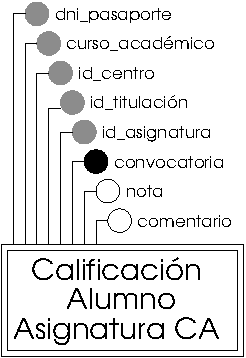
\includegraphics[]{07.Modelo_Entidad-Interrelacion/7.2.Analisis_Entidades/diagramas/cal_al_aca.pdf}
            \caption{Diagrama de la entidad Calificación Alumno Asignatura CA.}
            \label{diagramaCalAlACA}
            \end{center}
         \end{figure}

   \item[Descripción de los atributos propios] La entidad presenta los
   siguientes atributos propios:

   \begin{itemize}
    \item \textbf{convocatoria}
    \begin{itemize}
      \item \textbf{Definición:} Establece la convocatoria en la que el
      alumno se presenta a la asignatura.
      \item \textbf{Dominio:} Conjunto de caracteres alfanuméricos.
      \item \textbf{Carácter:} Obligatorio.
      \item \textbf{Ejemplo práctico:} febrero.
      \item \textbf{Información adicional:} Es clave primaria de la
      entidad. El dato lo introduce el usuario alumno al actualizar
      su información personal, o bien el usuario asesor si
      comprueba que la información no es correcta.
    \end{itemize}
    \item \textbf{nota}
    \begin{itemize}
      \item \textbf{Definición:} Establece la calificación obtenida por un
      alumno en una asignatura durante un curso académico.
      \item \textbf{Dominio:} Conjunto de reales positivos.
      \item \textbf{Carácter:} Opcional.
      \item \textbf{Ejemplo práctico:} 8,4.
      \item \textbf{Información adicional:} El dato lo introduce el
      usuario alumno al actualizar su información personal , o
      bien el usuario asesor si comprueba que la información no es
      correcta.
    \end{itemize}
    \item \textbf{comentario}
    \begin{itemize}
      \item \textbf{Definición:} Información extra que pueda ser
      interesante conocer.
      \item \textbf{Dominio:} Conjunto de caracteres alfanuméricos.
      \item \textbf{Carácter:} Opcional.
      \item \textbf{Ejemplo práctico:} Prácticas superadas.
      \item \textbf{Información adicional:} El dato lo introduce el
      usuario alumno al actualizar su información personal , o
      bien el usuario asesor si comprueba que la información no es
      correcta.
    \end{itemize}
   \end{itemize}

   \item[Ejemplo práctico]

   \item \begin{center}
            \begin{tabular}{ | l | l | }
            \hline
            \multicolumn{2}{ | c | }{\textbf{Tipo de entidad Calificación Alumno Asignatura CA}} \\
            \hline
            dni\_pasaporte & 01234567A \\
            \hline
            curso\_académico & 2008 \\
            \hline
            id\_centro & 15 \\
            \hline
            id\_titulación & 3\\
            \hline
            id\_asignatura & 17\\
            \hline
            convocatoria & febrero \\
            \hline
            nota & 8,4 \\
            \hline
            comentario & Prácticas superadas \\
            \hline
            \end{tabular}
         \end{center}
   \end{description}

   \subsection{Tipo de entidad Plantilla Entrevista Oficial}

   \begin{description}

   \item[Definición] Se refiere al objeto del mundo real: \emph{``Conjunto de
   preguntas que realiza un asesor en un momento determinado, de forma
   individual o grupal a los alumnos, en base a los documentos de entrevistas
   oficiales existentes''}.

   \item[Características] La entidad presenta las siguientes características:
      \begin{itemize}
         \item \textbf{Nombre:} Plantilla Entrevista Oficial.
         \item \textbf{Tipo:} Fuerte.
         \item \textbf{Número de atributos:} 3.
         \item \textbf{Atributo/s identificador/es principal/es:} id\_entrevista\_oficial.
         \item \textbf{Atributo/s identificador/es alternativo/s:} -
         \item \textbf{Atributo/s heredado/s:} -
      \end{itemize}

   \item[Diagrama] La figura \ref{diagramaPlantEntOfi} muestra el diagrama de la entidad.
   \item \begin{figure}[!ht]
            \begin{center}
            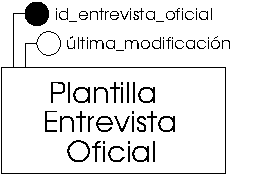
\includegraphics[]{07.Modelo_Entidad-Interrelacion/7.2.Analisis_Entidades/diagramas/plant_ent_ofi.pdf}
            \caption{Diagrama de la entidad Plantilla Entrevista Oficial.}
            \label{diagramaPlantEntOfi}
            \end{center}
         \end{figure}

   \item[Descripción de los atributos propios] La entidad presenta los
   siguientes atributos propios:

   \begin{itemize}
    \item \textbf{id\_entrevista\_oficial}
      \begin{itemize}
         \item \textbf{Definición:} Código que sirve como número identificativo
               para cada plantilla de entrevista oficial del sistema.
         \item \textbf{Dominio:} Números naturales.
         \item \textbf{Carácter:} Obligatorio.
         \item \textbf{Ejemplo práctico:} 24.
         \item \textbf{Información adicional:} El dato lo genera el sistema
               cuando se introduce una nueva plantilla de entrevista oficial en
               el sistema. Es la clave primaria.
      \end{itemize}
    \item \textbf{descripción}
      \begin{itemize}
         \item \textbf{Definición:} Establece una breve descripción que permite
         reconocer una plantilla de entrevista oficial del resto.
         \item \textbf{Dominio:} Conjunto de caracteres alfanuméricos.
         \item \textbf{Carácter:} Opcional.
         \item \textbf{Ejemplo práctico:} Plantilla de entrevista de ofertas de empleo.
         \item \textbf{Información adicional:} El dato lo introduce el
         usuario administrador al introducir una nueva plantilla de entrevista
         oficial en el sistema.
      \end{itemize}
    \item \textbf{última\_modificación}
      \begin{itemize}
         \item \textbf{Definición:} Establece el día, mes y año cuando se
            produjo la última modificación de la entidad.
         \item \textbf{Dominio:} Formato de fecha: dd/mm/aaaa.
         \item \textbf{Carácter:} Opcional.
         \item \textbf{Ejemplo práctico:} 02/02/2009.
         \item \textbf{Información adicional:} El dato lo genera el sistema
               cuando se modifica una plantilla de entrevista oficial en
               el sistema.
      \end{itemize}
   \end{itemize}

   \item[Ejemplo práctico]

   \item \begin{center}
            \begin{tabular}{ | l | l | }
            \hline
            \multicolumn{2}{ | c | }{\textbf{Tipo de entidad Plantilla Entrevista Oficial}} \\
            \hline
            id\_entrevista\_oficial & 24 \\
            \hline
            descripción & Plantilla de entrevista de ofertas de empleo \\
            \hline
            última\_modificación & 02/02/2009 \\
            \hline
            \end{tabular}
         \end{center}
   \end{description}

   \subsection{Tipo de entidad Pregunta Oficial}

   \begin{description}

   \item[Definición] Se refiere al objeto del mundo real: \emph{``Cuestión
   perteneciente a una plantilla de entrevista oficial planteada por el usuario
   asesor al usuario alumno''}.

   \item[Características] La entidad presenta las siguientes características:
      \begin{itemize}
         \item \textbf{Nombre:} Pregunta Oficial.
         \item \textbf{Tipo:} Débil por identificación con respecto a
         Plantilla Entrevista Oficial.
         \item \textbf{Número de atributos:} 3 propios y 1 heredado.
         \item \textbf{Atributo/s identificador/es principal/es:} id\_pregunta\_oficial.
         \item \textbf{Atributo/s identificador/es alternativo/s:} -
         \item \textbf{Atributo/s heredado/s:} id\_entrevista\_oficial del tipo
         de entidad Plantilla Entrevista Oficial.
      \end{itemize}

   \item[Diagrama] La figura \ref{diagramaPregOfi} muestra el diagrama de la entidad.
   \item \begin{figure}[!ht]
            \begin{center}
            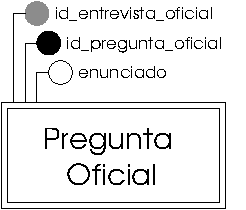
\includegraphics[]{07.Modelo_Entidad-Interrelacion/7.2.Analisis_Entidades/diagramas/preg_ofi.pdf}
            \caption{Diagrama de la entidad Pregunta Oficial.}
            \label{diagramaPregOfi}
            \end{center}
         \end{figure}

   \item[Descripción de los atributos propios] La entidad presenta los siguientes
   atributos propios:

   \begin{itemize}
    \item \textbf{id\_pregunta\_oficial}
      \begin{itemize}
         \item \textbf{Definición:} Código que sirve como número identificativo
               para cada pregunta oficial del sistema.
         \item \textbf{Dominio:} Números naturales.
         \item \textbf{Carácter:} Obligatorio.
         \item \textbf{Ejemplo práctico:} 55.
         \item \textbf{Información adicional:} El dato lo genera el sistema
               cuando se introduce una nueva pregunta oficial en el sistema. Es
               la clave primaria.
      \end{itemize}
   \item \textbf{enunciado}
      \begin{itemize}
         \item \textbf{Definición:} Cuestión perteneciente a una entrevista
         oficial, planteada a un alumno.
         \item \textbf{Dominio:} Conjunto de caracteres alfanuméricos.
         \item \textbf{Carácter:} Obligatorio.
         \item \textbf{Ejemplo práctico:} ¿Quién le ha informado de esta
         carrera?.
         \item \textbf{Información adicional:} El dato lo introduce el
         administrador principal al introducir una nueva pregunta oficial en el
         sistema.
      \end{itemize}
    \item \textbf{última\_modificación}
      \begin{itemize}
         \item \textbf{Definición:} Establece el día, mes y año cuando se
            produjo la última modificación de la entidad.
         \item \textbf{Dominio:} Formato de fecha: dd/mm/aaaa.
         \item \textbf{Carácter:} Opcional.
         \item \textbf{Ejemplo práctico:} 02/02/2009.
         \item \textbf{Información adicional:} El dato lo genera el sistema
               cuando se modifica una pregunta oficial en el sistema.
      \end{itemize}
   \end{itemize}

   \item[Ejemplo práctico]

   \item \begin{center}
            \begin{tabular}{ | l | l | }
            \hline
            \multicolumn{2}{ | c | }{\textbf{Tipo de entidad Pregunta Oficial}} \\
            \hline
            id\_entrevista\_oficial & 24 \\
            \hline
            id\_pregunta\_oficial & 55 \\
            \hline
            enunciado & ¿Quién le ha informado de esta carrera? \\
            \hline
            última\_modificación & 02/02/2009 \\
            \hline
            \end{tabular}
         \end{center}
   \end{description}

   \subsection{Tipo de entidad Reunión}

   \begin{description}

   \item[Definición] Se refiere al objeto del mundo real: \emph{``Encuentro,
   real o virtual, entre un usuario asesor y al menos un usuario alumno''}.

   \item[Características] La entidad presenta las siguientes características:
      \begin{itemize}
         \item \textbf{Nombre:} Pregunta Asesor.
         \item \textbf{Tipo:} Débil por identificación con respecto a
         Alumno Curso Académico.
         \item \textbf{Número de atributos:} 5 propios y 2 heredados.
         \item \textbf{Atributo/s identificador/es principal/es:} dni\_pasaporte
         junto con curso\_académico e id\_reunión.
         \item \textbf{Atributo/s identificador/es alternativo/s:} -
         \item \textbf{Atributo/s heredado/s:} dni\_pasaporte y curso\_académico
         del tipo de entidad Alumno Curso Académico.
      \end{itemize}

   \item[Diagrama] La figura \ref{diagramaReunion} muestra el diagrama de la entidad.
   \item \begin{figure}[!ht]
            \begin{center}
            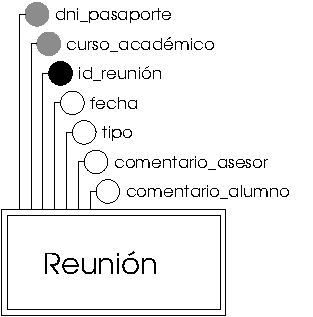
\includegraphics[]{07.Modelo_Entidad-Interrelacion/7.2.Analisis_Entidades/diagramas/reunion.pdf}
            \caption{Diagrama de la entidad Reunión.}
            \label{diagramaReunion}
            \end{center}
         \end{figure}

   \item[Descripción de los atributos propios] La entidad presenta los siguientes
   atributos propios:

   \begin{itemize}
    \item \textbf{id\_reunión}
      \begin{itemize}
         \item \textbf{Definición:} Código que sirve como número identificativo
               para cada reunión del sistema.
         \item \textbf{Dominio:} Números naturales.
         \item \textbf{Carácter:} Obligatorio.
         \item \textbf{Ejemplo práctico:} 121.
         \item \textbf{Información adicional:} El dato lo genera el sistema
               cuando se introduce una nueva reunión en el sistema. Es la clave
               primaria.
      \end{itemize}
    \item \textbf{fecha}
      \begin{itemize}
        \item \textbf{Definición:} Establece el día, mes y año cuando se
        produce la reunión.
        \item \textbf{Dominio:} Formato de fecha: dd/mm/aaaa.
        \item \textbf{Carácter:} Opcional.
        \item \textbf{Ejemplo práctico:} 01/01/2009.
        \item \textbf{Información adicional:} El dato lo introduce el
        usuario asesor cuando introduce una nueva reunión en el sistema.
      \end{itemize}
    \item \textbf{tipo}
      \begin{itemize}
        \item \textbf{Definición:} Establece el tipo de reunión realizada,
        ya sea grupal o individual.
        \item \textbf{Dominio:} Unos de los valores: grupal o individual.
        \item \textbf{Carácter:} Obligatorio.
        \item \textbf{Ejemplo práctico:} Individual.
        \item \textbf{Información adicional:} El dato lo introduce el
         usuario asesor cuando introduce una nueva reunión en el sistema.
      \end{itemize}
    \item \textbf{comentario\_asesor}
          \begin{itemize}
            \item \textbf{Definición:} Información extra que pueda ser
            interesante conocer por parte del usuario asesor.
            \item \textbf{Dominio:} Conjunto de caracteres alfanuméricos.
            \item \textbf{Carácter:} Opcional.
            \item \textbf{Ejemplo práctico:} Pendiente de entregar el proyecto.
            \item \textbf{Información adicional:} El dato lo introduce el
            usuario asesor al llevarse a cabo una reunión.
         \end{itemize}
    \item \textbf{comentario\_alumno}
          \begin{itemize}
            \item \textbf{Definición:} Información extra que pueda ser
            interesante conocer por parte del usuario alumno.
            \item \textbf{Dominio:} Conjunto de caracteres alfanuméricos.
            \item \textbf{Carácter:} Opcional.
            \item \textbf{Ejemplo práctico:} Terminando el manual técnico.
            \item \textbf{Información adicional:} El dato lo introduce el
            usuario alumno al llevarse a cabo una reunión.
         \end{itemize}
   \end{itemize}

   \item[Ejemplo práctico]

   \item \begin{center}
            \begin{tabular}{ | l | l | }
            \hline
            \multicolumn{2}{ | c | }{\textbf{Tipo de entidad Reunión}} \\
            \hline
            dni\_pasaporte & 01234567A \\
            \hline
            curso\_académico & 2008 \\
            \hline
            id\_reunión & 121 \\
            \hline
            fecha & 01/01/2009 \\
            \hline
            tipo & Individual \\
            \hline
            comentario\_asesor & Pendiente de entregar el proyecto \\
            \hline
            comentario\_alumno & Terminando el manual técnico \\
            \hline
            \end{tabular}
         \end{center}
   \end{description}

